% =============================================================================
%  Breadcrumbs
%  Blockchain Olympiad submission, Team CookieMonsters, United International
%  University.
%
%  HOW TO COMPILE
%    Upload main.tex and ref.bib to Overleaf. Set the compiler to pdfLaTeX.
%    Overleaf runs BibTeX automatically. Nothing else is needed: every figure
%    is drawn in TikZ inside this file, so there are no image files to upload.
%
%  >>> EDIT THE TEAM BLOCK BELOW BEFORE SUBMITTING <<<
% =============================================================================
\documentclass[11pt,border=6pt,varwidth=20cm]{standalone}

% ---- team details: replace the bracketed placeholders -----------------------
\newcommand{\TeamName}{CookieMonsters}
\newcommand{\TeamInstitution}{United International University, Dhaka, Bangladesh}
\newcommand{\TeamMembers}{Ahbab, Ruhi, Rohan, Ishmam, Adnan}
\newcommand{\TeamCategory}{Undergraduate}
\newcommand{\TeamContact}{mkhan223869@bscse.uiu.ac.bd}
% -----------------------------------------------------------------------------

\usepackage[T1]{fontenc}
\usepackage[utf8]{inputenc}
\usepackage{lmodern}

\usepackage{amsmath,amssymb}
\usepackage{graphicx}
\usepackage{xcolor}
\usepackage{booktabs}
\usepackage{tabularx}
\usepackage{array}
\usepackage{longtable}
\usepackage{caption}
\usepackage{enumitem}
\usepackage{titlesec}

\usepackage{tikz}
\usepackage{pgfplots}
\usepackage{algorithm}
\usepackage{algpseudocode}



\usetikzlibrary{positioning,shapes.geometric,arrows.meta,calc,fit,backgrounds}
\pgfplotsset{compat=1.18}

% ---- palette (colour-blind safe, prints correctly in greyscale) -------------
\definecolor{tcblue}{HTML}{2563EB}
\definecolor{tcorange}{HTML}{E8710A}
\definecolor{tcgreen}{HTML}{059669}
\definecolor{tcgrey}{HTML}{6B7280}
\definecolor{tctext}{HTML}{111827}
\definecolor{tcline}{HTML}{E5E7EB}
\definecolor{tcbg}{HTML}{F7F8FA}


\captionsetup{font=small,labelfont={bf,sf}}
\setlength{\parskip}{0.35em}
\renewcommand{\arraystretch}{1.18}




\newcolumntype{Y}{>{\raggedright\arraybackslash}X}
\newcommand{\est}{\textsuperscript{\textdagger}}

% ---- the logo, drawn rather than imported ----------------------------------
% A trail of marks, each one larger and more definite than the last, ending in
% the verified record. Drawn rather than imported so the file stays standalone.
\newcommand{\bclogo}[1][1.0]{%
\begin{tikzpicture}[scale=#1,every node/.style={transform shape}]
  \node[regular polygon,regular polygon sides=6,draw=tcblue,line width=1.5pt,
        minimum size=2.35cm,rotate=90] (hex) at (0,0) {};
  \draw[tcgrey!45,line width=1.0pt,dash pattern=on 1pt off 2.6pt,line cap=round]
        (-0.53,-0.36) -- (0.53,0.36);
  \fill[tcgrey!55] (-0.53,-0.36) circle (0.085);
  \fill[tcgrey]    (-0.27,-0.17) circle (0.110);
  \fill[tcblue]    ( 0.00, 0.00) circle (0.135);
  \fill[tcorange]  ( 0.27, 0.17) circle (0.155);
  \fill[tcgreen]   ( 0.53, 0.36) circle (0.180);
\end{tikzpicture}}

\begin{document}
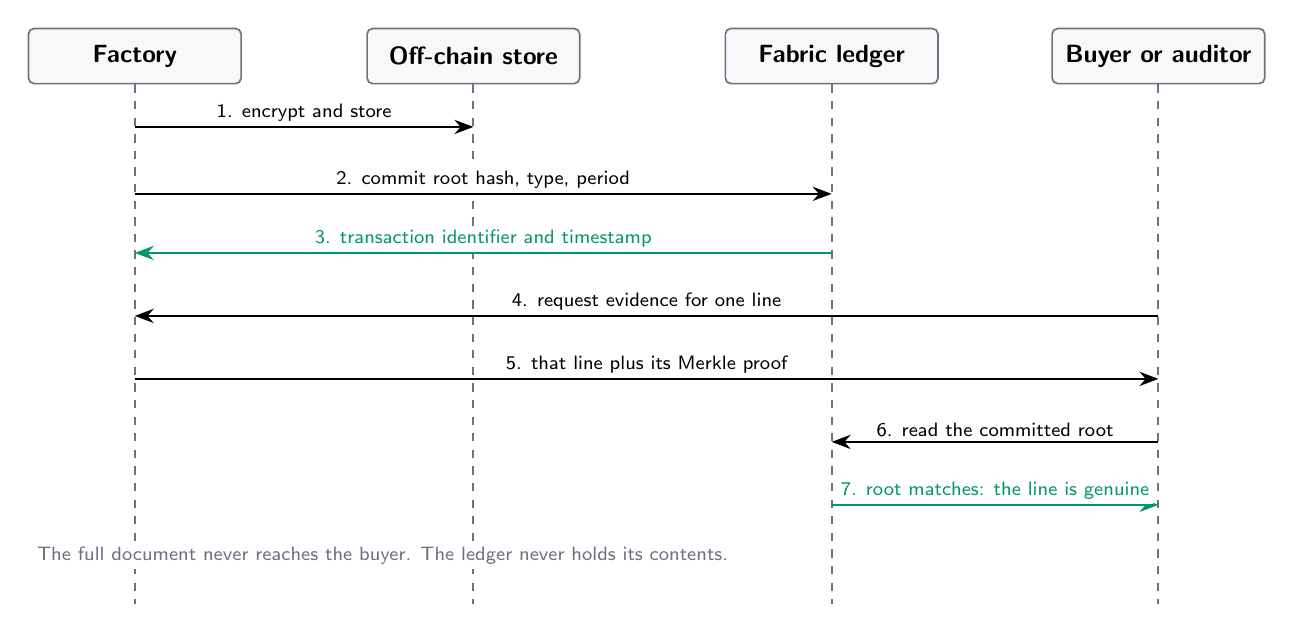
\begin{tikzpicture}[font=\sffamily\small,
  ll/.style={draw=tcgrey,line width=0.7pt,dashed},
  hd/.style={rounded corners=2pt,draw=tcgrey,fill=tcbg,line width=0.6pt,
             minimum height=0.7cm,minimum width=2.7cm,align=center,font=\sffamily\small\bfseries},
  msg/.style={-{Stealth[length=2.4mm]},line width=0.8pt},
  st/.style={font=\sffamily\scriptsize,align=center,fill=white,inner sep=1.5pt}]

\node[hd] (F) at (1.45,0)  {Factory};
\node[hd] (S) at (5.75,0)  {Off-chain store};
\node[hd] (L) at (10.3,0)  {Fabric ledger};
\node[hd] (B) at (14.45,0) {Buyer or auditor};
\foreach \n in {F,S,L,B} \draw[ll] (\n.south) -- ++(0,-6.6);

\draw[msg] (1.45,-0.9)  -- node[st,above]{1. encrypt and store} (5.75,-0.9);
\draw[msg] (1.45,-1.75) -- node[st,above]{2. commit root hash, type, period} (10.3,-1.75);
\draw[msg,tcgreen] (10.3,-2.5) -- node[st,above]{3. transaction identifier and timestamp} (1.45,-2.5);
\draw[msg] (14.45,-3.3) -- node[st,above]{4. request evidence for one line} (1.45,-3.3);
\draw[msg] (1.45,-4.1)  -- node[st,above]{5. that line plus its Merkle proof} (14.45,-4.1);
\draw[msg] (14.45,-4.9) -- node[st,above]{6. read the committed root} (10.3,-4.9);
\draw[msg,tcgreen] (10.3,-5.7) -- node[st,above]{7. root matches: the line is genuine} (14.45,-5.7);
\node[st,text=tcgrey,anchor=west] at (0.15,-6.35)
  {The full document never reaches the buyer. The ledger never holds its contents.};
\end{tikzpicture}
\end{document}
